\documentclass[border=4pt]{standalone}

\usepackage{amsmath}
\usepackage{tikz}
\usepackage{mathdots}
\usepackage{yhmath}
\usepackage{cancel}
\usepackage{color}
\usepackage{siunitx}
\usepackage{array}
\usepackage{multirow}
\usepackage{amssymb}
\usepackage{gensymb}
\usepackage{tabularx}
\usepackage{booktabs}
\usetikzlibrary{fadings}
\usetikzlibrary{patterns}


\begin{document}
 

\tikzset{every picture/.style={line width=0.75pt}} %set default line width to 0.75pt        

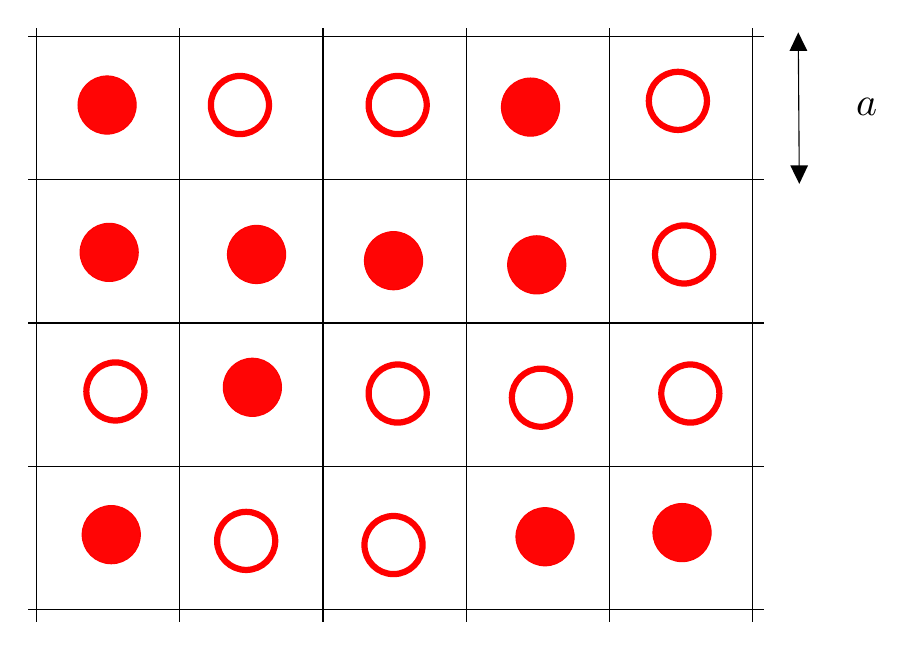
\begin{tikzpicture}[x=0.75pt,y=0.75pt,yscale=-1,xscale=1]
%uncomment if require: \path (0,656); %set diagram left start at 0, and has height of 656

%Shape: Grid [id:dp07999700806031962] 
\draw  [draw opacity=0] (100,112) -- (454.5,112) -- (454.5,398) -- (100,398) -- cycle ; \draw   (104,112) -- (104,398)(173,112) -- (173,398)(242,112) -- (242,398)(311,112) -- (311,398)(380,112) -- (380,398)(449,112) -- (449,398) ; \draw   (100,116) -- (454.5,116)(100,185) -- (454.5,185)(100,254) -- (454.5,254)(100,323) -- (454.5,323)(100,392) -- (454.5,392) ; \draw    ;
%Shape: Circle [id:dp05581530145302649] 
\draw  [color={rgb, 255:red, 255; green, 0; blue, 0 }  ,draw opacity=1 ][fill={rgb, 255:red, 255; green, 5; blue, 5 }  ,fill opacity=1 ] (124,149) .. controls (124,141.27) and (130.27,135) .. (138,135) .. controls (145.73,135) and (152,141.27) .. (152,149) .. controls (152,156.73) and (145.73,163) .. (138,163) .. controls (130.27,163) and (124,156.73) .. (124,149) -- cycle ;
%Shape: Circle [id:dp3826378738505667] 
\draw  [color={rgb, 255:red, 255; green, 0; blue, 0 }  ,draw opacity=1 ][fill={rgb, 255:red, 255; green, 5; blue, 5 }  ,fill opacity=0 ][line width=2.25]  (188,149) .. controls (188,141.27) and (194.27,135) .. (202,135) .. controls (209.73,135) and (216,141.27) .. (216,149) .. controls (216,156.73) and (209.73,163) .. (202,163) .. controls (194.27,163) and (188,156.73) .. (188,149) -- cycle ;
%Shape: Circle [id:dp5901037269104972] 
\draw  [color={rgb, 255:red, 255; green, 0; blue, 0 }  ,draw opacity=1 ][fill={rgb, 255:red, 255; green, 5; blue, 5 }  ,fill opacity=1 ] (125,220) .. controls (125,212.27) and (131.27,206) .. (139,206) .. controls (146.73,206) and (153,212.27) .. (153,220) .. controls (153,227.73) and (146.73,234) .. (139,234) .. controls (131.27,234) and (125,227.73) .. (125,220) -- cycle ;
%Shape: Circle [id:dp8116731619355144] 
\draw  [color={rgb, 255:red, 255; green, 0; blue, 0 }  ,draw opacity=1 ][fill={rgb, 255:red, 255; green, 5; blue, 5 }  ,fill opacity=1 ] (194,285) .. controls (194,277.27) and (200.27,271) .. (208,271) .. controls (215.73,271) and (222,277.27) .. (222,285) .. controls (222,292.73) and (215.73,299) .. (208,299) .. controls (200.27,299) and (194,292.73) .. (194,285) -- cycle ;
%Shape: Circle [id:dp04600561272899939] 
\draw  [color={rgb, 255:red, 255; green, 0; blue, 0 }  ,draw opacity=1 ][fill={rgb, 255:red, 255; green, 5; blue, 5 }  ,fill opacity=1 ] (126,356) .. controls (126,348.27) and (132.27,342) .. (140,342) .. controls (147.73,342) and (154,348.27) .. (154,356) .. controls (154,363.73) and (147.73,370) .. (140,370) .. controls (132.27,370) and (126,363.73) .. (126,356) -- cycle ;
%Shape: Circle [id:dp5564199220147412] 
\draw  [color={rgb, 255:red, 255; green, 0; blue, 0 }  ,draw opacity=1 ][fill={rgb, 255:red, 255; green, 5; blue, 5 }  ,fill opacity=1 ] (401,355) .. controls (401,347.27) and (407.27,341) .. (415,341) .. controls (422.73,341) and (429,347.27) .. (429,355) .. controls (429,362.73) and (422.73,369) .. (415,369) .. controls (407.27,369) and (401,362.73) .. (401,355) -- cycle ;
%Shape: Circle [id:dp24617845851636] 
\draw  [color={rgb, 255:red, 255; green, 0; blue, 0 }  ,draw opacity=1 ][fill={rgb, 255:red, 255; green, 5; blue, 5 }  ,fill opacity=1 ] (335,357) .. controls (335,349.27) and (341.27,343) .. (349,343) .. controls (356.73,343) and (363,349.27) .. (363,357) .. controls (363,364.73) and (356.73,371) .. (349,371) .. controls (341.27,371) and (335,364.73) .. (335,357) -- cycle ;
%Shape: Circle [id:dp4729644813439582] 
\draw  [color={rgb, 255:red, 255; green, 0; blue, 0 }  ,draw opacity=1 ][fill={rgb, 255:red, 255; green, 5; blue, 5 }  ,fill opacity=1 ] (196,221) .. controls (196,213.27) and (202.27,207) .. (210,207) .. controls (217.73,207) and (224,213.27) .. (224,221) .. controls (224,228.73) and (217.73,235) .. (210,235) .. controls (202.27,235) and (196,228.73) .. (196,221) -- cycle ;
%Shape: Circle [id:dp15295592273906244] 
\draw  [color={rgb, 255:red, 255; green, 0; blue, 0 }  ,draw opacity=1 ][fill={rgb, 255:red, 255; green, 5; blue, 5 }  ,fill opacity=1 ] (262,224) .. controls (262,216.27) and (268.27,210) .. (276,210) .. controls (283.73,210) and (290,216.27) .. (290,224) .. controls (290,231.73) and (283.73,238) .. (276,238) .. controls (268.27,238) and (262,231.73) .. (262,224) -- cycle ;
%Shape: Circle [id:dp6041188603097198] 
\draw  [color={rgb, 255:red, 255; green, 0; blue, 0 }  ,draw opacity=1 ][fill={rgb, 255:red, 255; green, 5; blue, 5 }  ,fill opacity=1 ] (331,226) .. controls (331,218.27) and (337.27,212) .. (345,212) .. controls (352.73,212) and (359,218.27) .. (359,226) .. controls (359,233.73) and (352.73,240) .. (345,240) .. controls (337.27,240) and (331,233.73) .. (331,226) -- cycle ;
%Shape: Circle [id:dp43865504980090897] 
\draw  [color={rgb, 255:red, 255; green, 0; blue, 0 }  ,draw opacity=1 ][fill={rgb, 255:red, 255; green, 5; blue, 5 }  ,fill opacity=1 ] (328,150) .. controls (328,142.27) and (334.27,136) .. (342,136) .. controls (349.73,136) and (356,142.27) .. (356,150) .. controls (356,157.73) and (349.73,164) .. (342,164) .. controls (334.27,164) and (328,157.73) .. (328,150) -- cycle ;
%Shape: Circle [id:dp19035591897168014] 
\draw  [color={rgb, 255:red, 255; green, 0; blue, 0 }  ,draw opacity=1 ][fill={rgb, 255:red, 255; green, 5; blue, 5 }  ,fill opacity=0 ][line width=2.25]  (264,149) .. controls (264,141.27) and (270.27,135) .. (278,135) .. controls (285.73,135) and (292,141.27) .. (292,149) .. controls (292,156.73) and (285.73,163) .. (278,163) .. controls (270.27,163) and (264,156.73) .. (264,149) -- cycle ;
%Shape: Circle [id:dp017907746004278913] 
\draw  [color={rgb, 255:red, 255; green, 0; blue, 0 }  ,draw opacity=1 ][fill={rgb, 255:red, 255; green, 5; blue, 5 }  ,fill opacity=0 ][line width=2.25]  (399,147) .. controls (399,139.27) and (405.27,133) .. (413,133) .. controls (420.73,133) and (427,139.27) .. (427,147) .. controls (427,154.73) and (420.73,161) .. (413,161) .. controls (405.27,161) and (399,154.73) .. (399,147) -- cycle ;
%Shape: Circle [id:dp31658426949621865] 
\draw  [color={rgb, 255:red, 255; green, 0; blue, 0 }  ,draw opacity=1 ][fill={rgb, 255:red, 255; green, 5; blue, 5 }  ,fill opacity=0 ][line width=2.25]  (402,221) .. controls (402,213.27) and (408.27,207) .. (416,207) .. controls (423.73,207) and (430,213.27) .. (430,221) .. controls (430,228.73) and (423.73,235) .. (416,235) .. controls (408.27,235) and (402,228.73) .. (402,221) -- cycle ;
%Shape: Circle [id:dp33086423585565194] 
\draw  [color={rgb, 255:red, 255; green, 0; blue, 0 }  ,draw opacity=1 ][fill={rgb, 255:red, 255; green, 5; blue, 5 }  ,fill opacity=0 ][line width=2.25]  (405,288) .. controls (405,280.27) and (411.27,274) .. (419,274) .. controls (426.73,274) and (433,280.27) .. (433,288) .. controls (433,295.73) and (426.73,302) .. (419,302) .. controls (411.27,302) and (405,295.73) .. (405,288) -- cycle ;
%Shape: Circle [id:dp5002532190079865] 
\draw  [color={rgb, 255:red, 255; green, 0; blue, 0 }  ,draw opacity=1 ][fill={rgb, 255:red, 255; green, 5; blue, 5 }  ,fill opacity=0 ][line width=2.25]  (191,359) .. controls (191,351.27) and (197.27,345) .. (205,345) .. controls (212.73,345) and (219,351.27) .. (219,359) .. controls (219,366.73) and (212.73,373) .. (205,373) .. controls (197.27,373) and (191,366.73) .. (191,359) -- cycle ;
%Shape: Circle [id:dp7978217342362601] 
\draw  [color={rgb, 255:red, 255; green, 0; blue, 0 }  ,draw opacity=1 ][fill={rgb, 255:red, 255; green, 5; blue, 5 }  ,fill opacity=0 ][line width=2.25]  (333,290) .. controls (333,282.27) and (339.27,276) .. (347,276) .. controls (354.73,276) and (361,282.27) .. (361,290) .. controls (361,297.73) and (354.73,304) .. (347,304) .. controls (339.27,304) and (333,297.73) .. (333,290) -- cycle ;
%Shape: Circle [id:dp6707317902863159] 
\draw  [color={rgb, 255:red, 255; green, 0; blue, 0 }  ,draw opacity=1 ][fill={rgb, 255:red, 255; green, 5; blue, 5 }  ,fill opacity=0 ][line width=2.25]  (264,288) .. controls (264,280.27) and (270.27,274) .. (278,274) .. controls (285.73,274) and (292,280.27) .. (292,288) .. controls (292,295.73) and (285.73,302) .. (278,302) .. controls (270.27,302) and (264,295.73) .. (264,288) -- cycle ;
%Shape: Circle [id:dp9732877617922888] 
\draw  [color={rgb, 255:red, 255; green, 0; blue, 0 }  ,draw opacity=1 ][fill={rgb, 255:red, 255; green, 5; blue, 5 }  ,fill opacity=0 ][line width=2.25]  (262,361) .. controls (262,353.27) and (268.27,347) .. (276,347) .. controls (283.73,347) and (290,353.27) .. (290,361) .. controls (290,368.73) and (283.73,375) .. (276,375) .. controls (268.27,375) and (262,368.73) .. (262,361) -- cycle ;
%Shape: Circle [id:dp47363620907663107] 
\draw  [color={rgb, 255:red, 255; green, 0; blue, 0 }  ,draw opacity=1 ][fill={rgb, 255:red, 255; green, 5; blue, 5 }  ,fill opacity=0 ][line width=2.25]  (128,287) .. controls (128,279.27) and (134.27,273) .. (142,273) .. controls (149.73,273) and (156,279.27) .. (156,287) .. controls (156,294.73) and (149.73,301) .. (142,301) .. controls (134.27,301) and (128,294.73) .. (128,287) -- cycle ;
%Straight Lines [id:da6668323367252631] 
\draw    (471.01,116) -- (471.49,185) ;
\draw [shift={(471.5,187)}, rotate = 269.61] [fill={rgb, 255:red, 0; green, 0; blue, 0 }  ][line width=0.75]  [draw opacity=0] (8.93,-4.29) -- (0,0) -- (8.93,4.29) -- cycle    ;
\draw [shift={(471,114)}, rotate = 89.61] [fill={rgb, 255:red, 0; green, 0; blue, 0 }  ][line width=0.75]  [draw opacity=0] (8.93,-4.29) -- (0,0) -- (8.93,4.29) -- cycle    ;

% Text Node
\draw (504,150) node [scale=1.44]  {$a$};


\end{tikzpicture}

\end{document}
